\subsection{Tinyworld2}\label[secc]{tinyworld2}
The Tinyworld2 environment is constructed to study how obstacles affect the configuration generated by Algorithm \ref{alg:alg1}.

The results of a simulation for 3 agents without active dispersion ($k_{1} = 0$) are shown in \Crefrange{fig:3_agnt_tw2_k_1_0_distr}{fig:3_agnt_tw2_evolution}.
\Crefrange{fig:6_agnt_tw2_k_1_0_distr}{fig:6_agnt_tw2_evolution} show the results of a simulation of 6 agents without active dispersion.

The results generated by Algorithm \ref{alg:alg1} when applying active dispersion ($k_{1} = 1$, $k_{1} = 2$) and running simulations for 3 and 6 agents 
are shown in \Crefrange{fig:3_agnt_tw2_k_1_1_k_2_1_distr}{fig:3_agnt_tw2_evolution_active} and \Crefrange{fig:6_agnt_tw2_k_1_1_k_2_1_distr}{fig:6_agnt_tw2_evolution_active} respectively.
\begin{figure}[H]
  \centering
  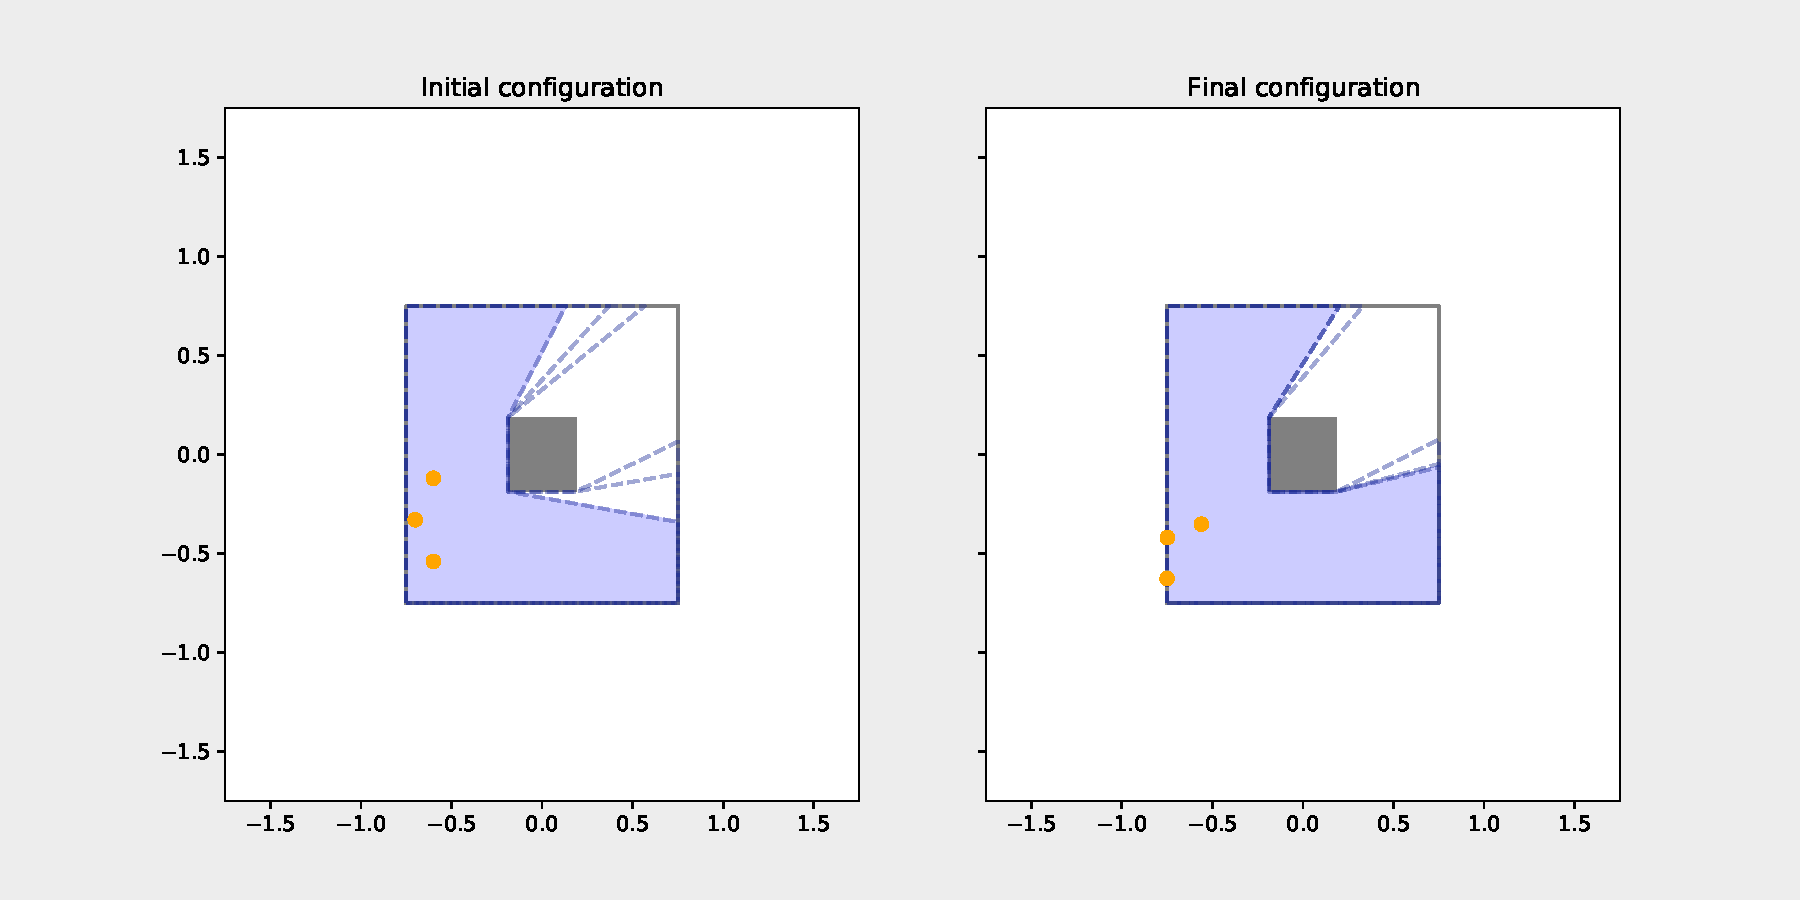
\includegraphics[width=\textwidth]{figs/tinyworld2_3_agnt_k_1_0_k_2_1_distr.pdf}
  \caption{Inital and final configuration of 3 agents in the Tinyworld2 environment with $k_{1} = 0$ (no active dispersion).}
  \label{fig:3_agnt_tw2_k_1_0_distr}
\end{figure}
\begin{figure}[H]
  \centering
  \begin{subfigure}[t]{0.5\textwidth}
    \centering
    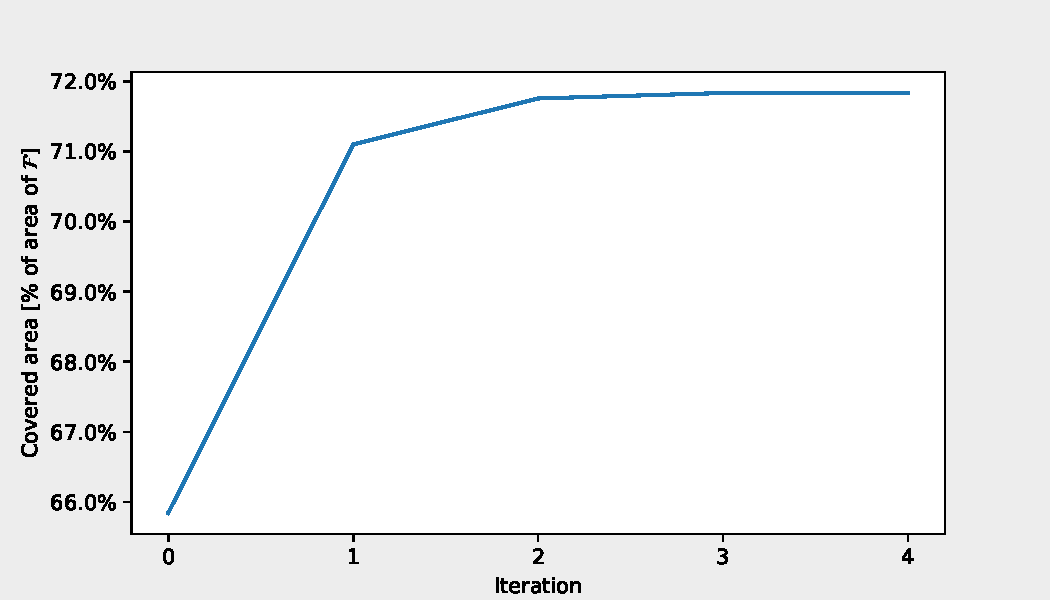
\includegraphics[width=\textwidth]{figs/tinyworld2_3_agnt_k_1_0_k_2_1_area_traj.pdf}
    \caption{Coverage evolution for 3 agents in the Tinyworld2 environment with $k_{1} = 0$ (no active dispersion).}
    \label{fig:3_agnt_tw2_k_1_0_a_traj}
  \end{subfigure}%
  ~ 
  \begin{subfigure}[t]{0.5\textwidth}
    \centering
    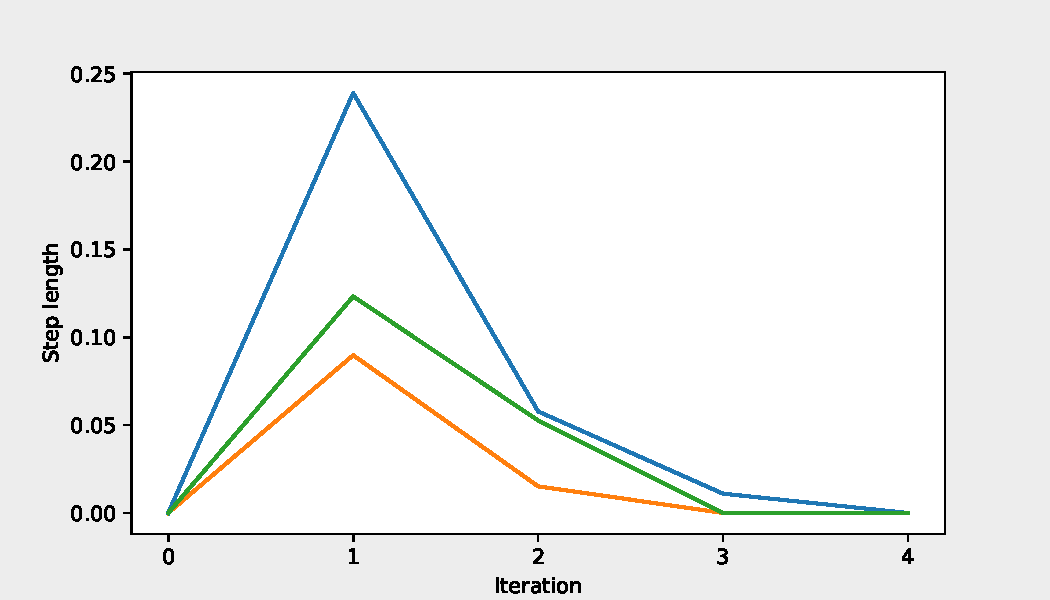
\includegraphics[width=\textwidth]{figs/tinyworld2_3_agnt_k_1_0_k_2_1_step_traj.pdf}
    \caption{Step length evolution for 3 agents in the Tinyworld2 environment with $k_{1} = 0$ (no active dispersion).}
    \label{fig:3_agnt_tw2_k_1_0_s_traj}
  \end{subfigure}
  \caption{Coverage percentage and step length evolution for 3 agents in the Tinyworld2 environment when no active dispersion is used.}
  \label{fig:3_agnt_tw2_evolution}
\end{figure}


\begin{figure}[H]
  \centering
  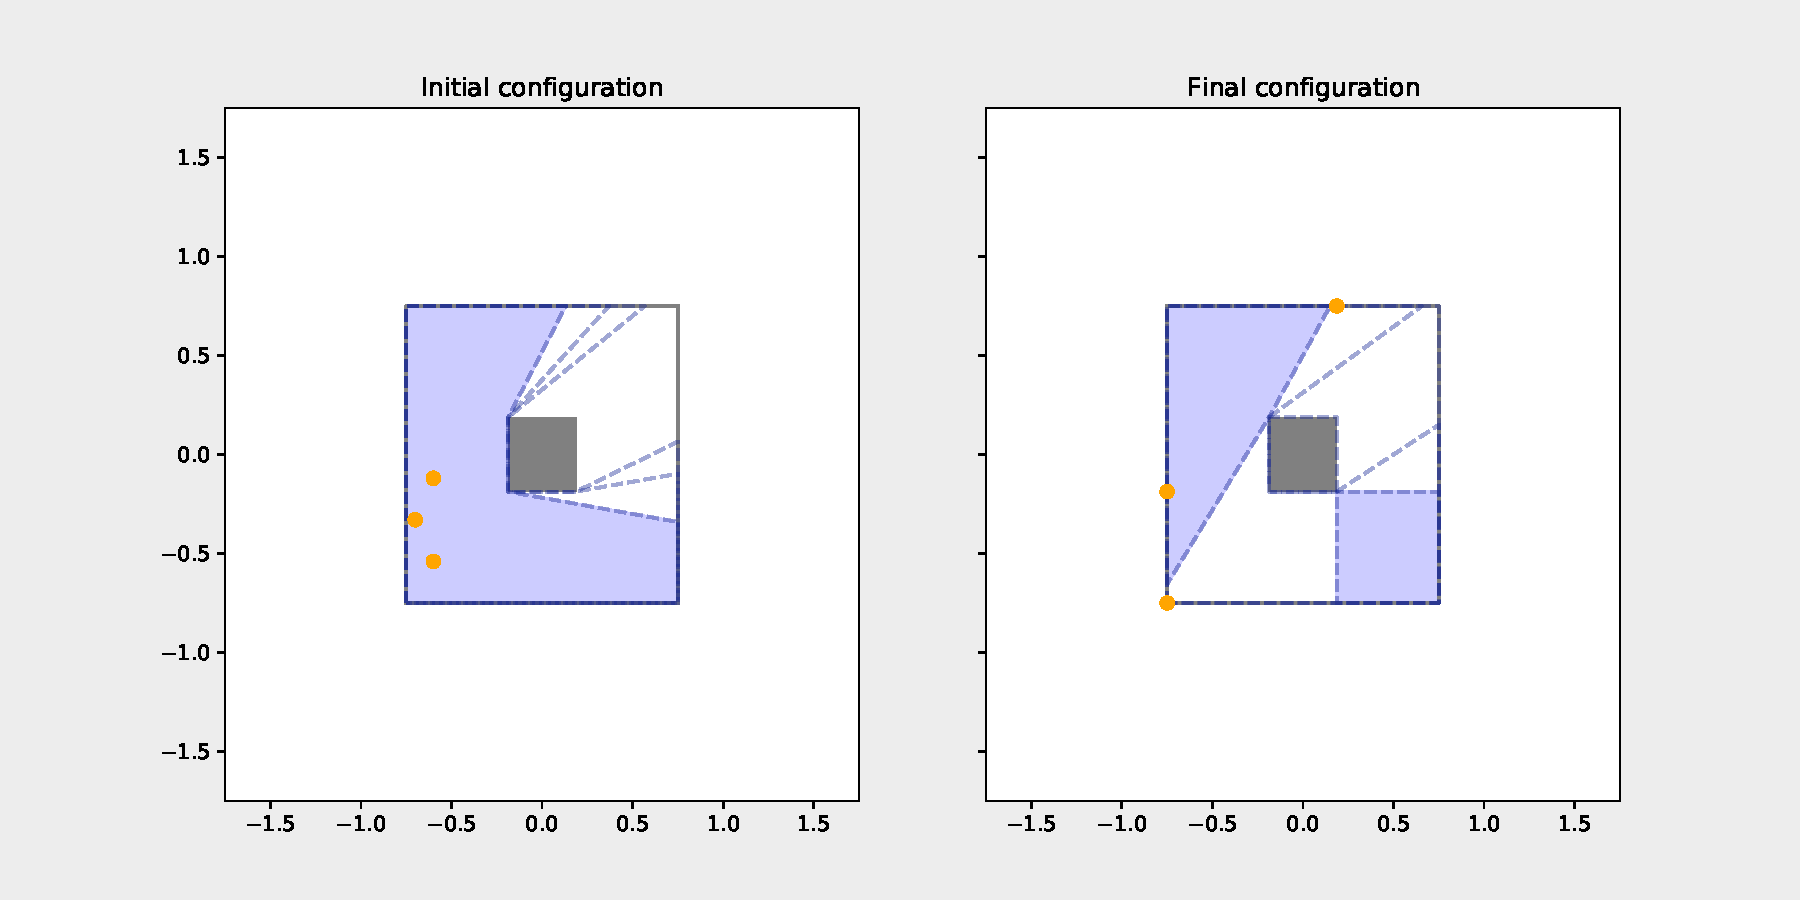
\includegraphics[width=\textwidth]{figs/tinyworld2_3_agnt_k_1_1_k_2_1_distr.pdf}
  \caption{Inital and final configuration of 3 agents in the Tinyworld2 environment with $k_{1} = k_{2} = 1$ (active dispersion).}
  \label{fig:3_agnt_tw2_k_1_1_k_2_1_distr}
\end{figure}
\begin{figure}[H]
  \centering
  \begin{subfigure}[t]{0.5\textwidth}
    \centering
    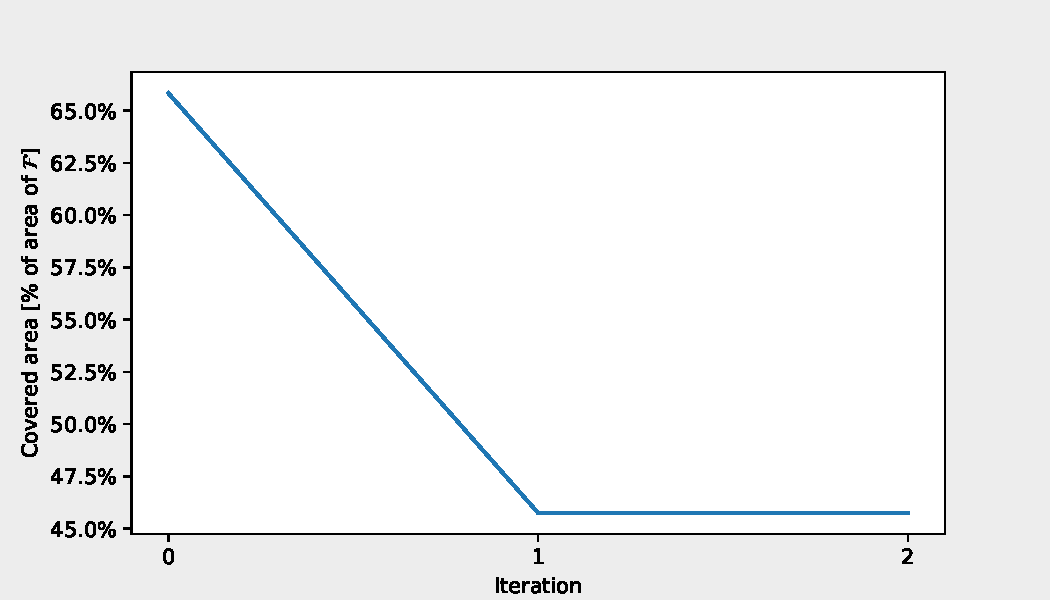
\includegraphics[width=\textwidth]{figs/tinyworld2_3_agnt_k_1_1_k_2_1_area_traj.pdf}
    \caption{Coverage evolution for 3 agents in the Tinyworld2 environment with $k_{1} = k_{2} = 1$ (active dispersion).}
    \label{fig:3_agnt_tw2_k_1_1_a_traj}
  \end{subfigure}%
  ~ 
  \begin{subfigure}[t]{0.5\textwidth}
    \centering
    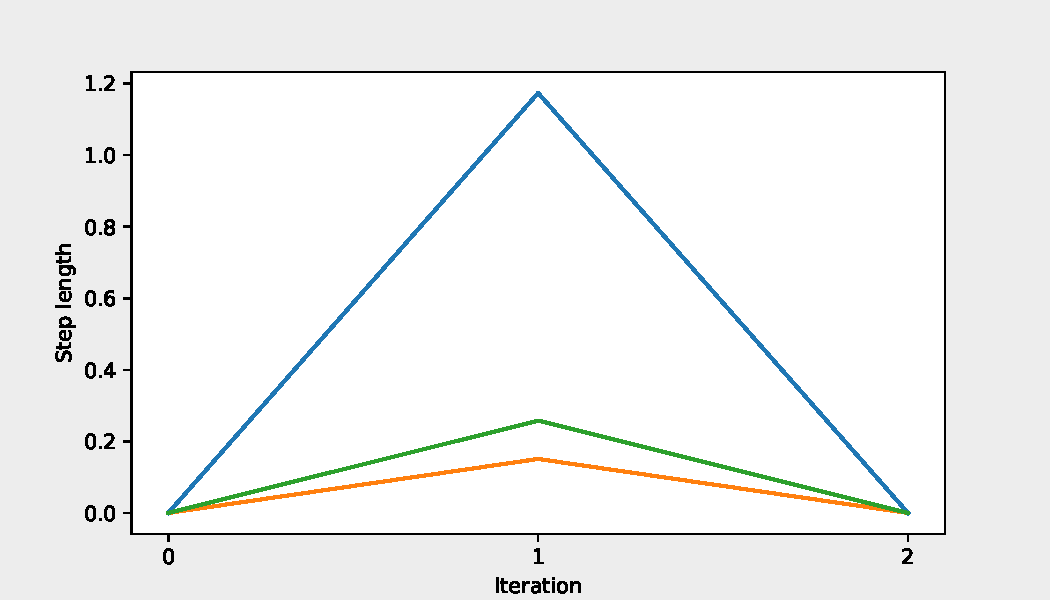
\includegraphics[width=\textwidth]{figs/tinyworld2_3_agnt_k_1_1_k_2_1_step_traj.pdf}
    \caption{Step length evolution for 3 agents in the Tinyworld2 environment with $k_{1} = k_{2} = 1$ (active dispersion).}
    \label{fig:3_agnt_tw2_k_1_1_s_traj}
  \end{subfigure}
  \caption{Coverage percentage and step length evolution for 3 agents in the Tinyworld2 environment when active dispersion is used.}
  \label{fig:3_agnt_tw2_evolution_active}
\end{figure}

\begin{figure}[H]
  \centering
  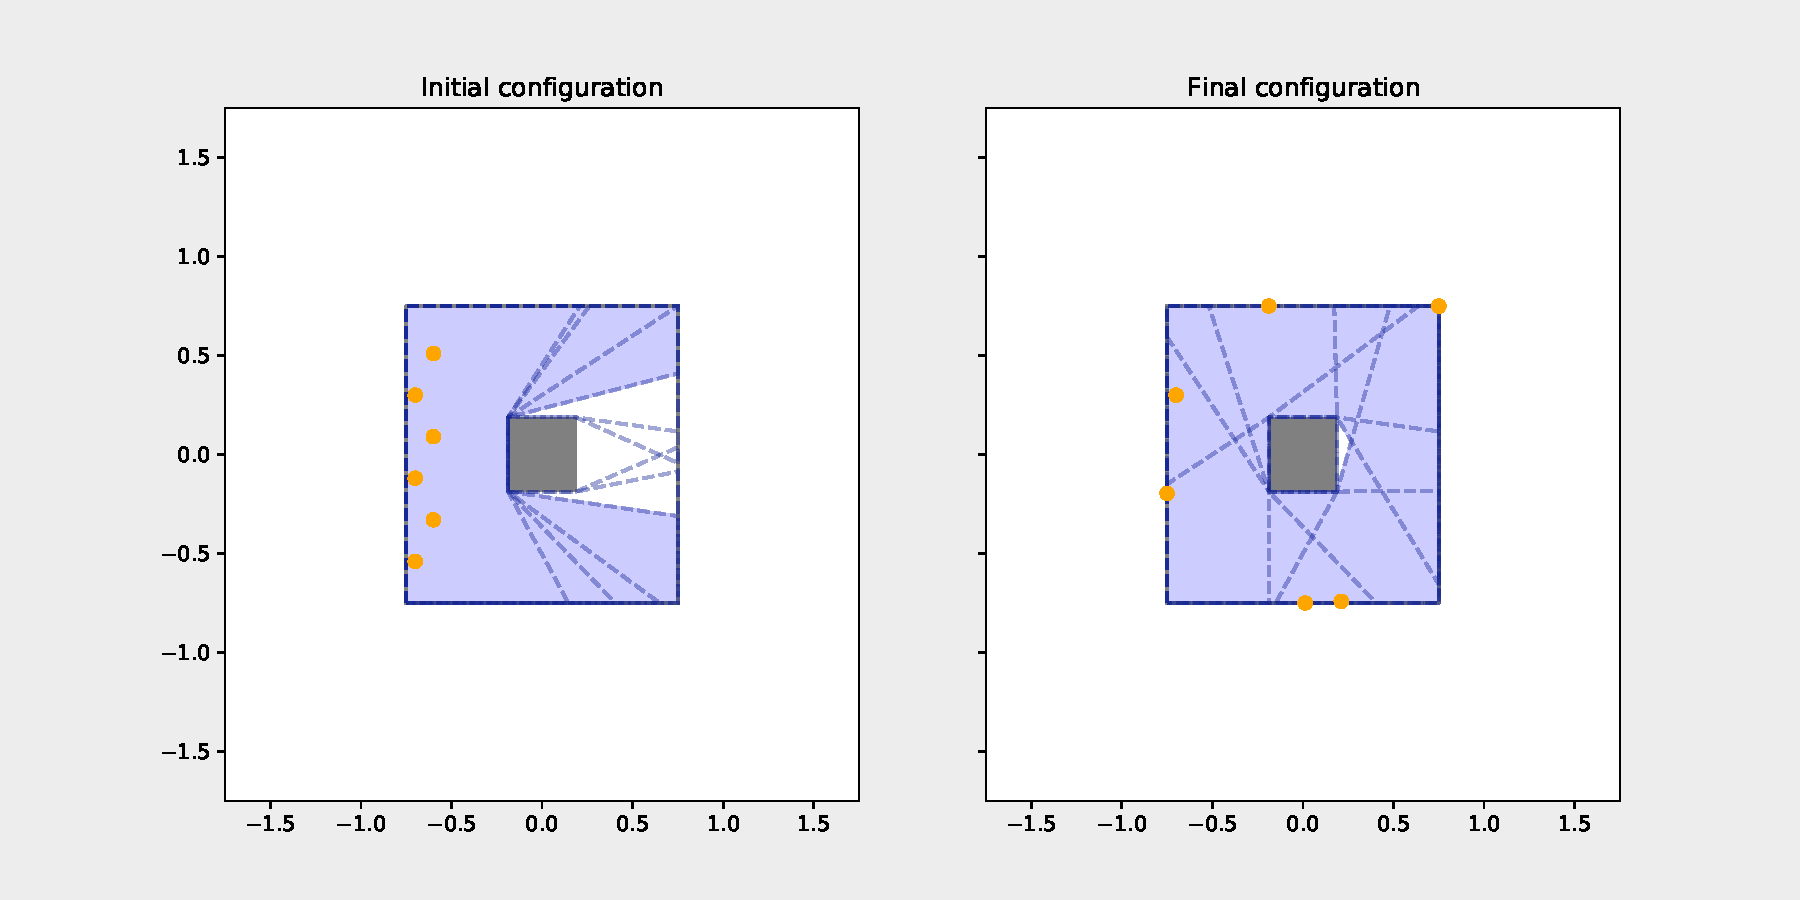
\includegraphics[width=\textwidth]{figs/tinyworld2_6_agnt_k_1_0_k_2_1_distr.pdf}
  \caption{Inital and final configuration of 6 agents in the Tinyworld2 environment with $k_{1} = 0$ (no active dispersion).}
  \label{fig:6_agnt_tw2_k_1_0_distr}
\end{figure}
\begin{figure}[H]
  \centering
  \begin{subfigure}[t]{0.5\textwidth}
    \centering
    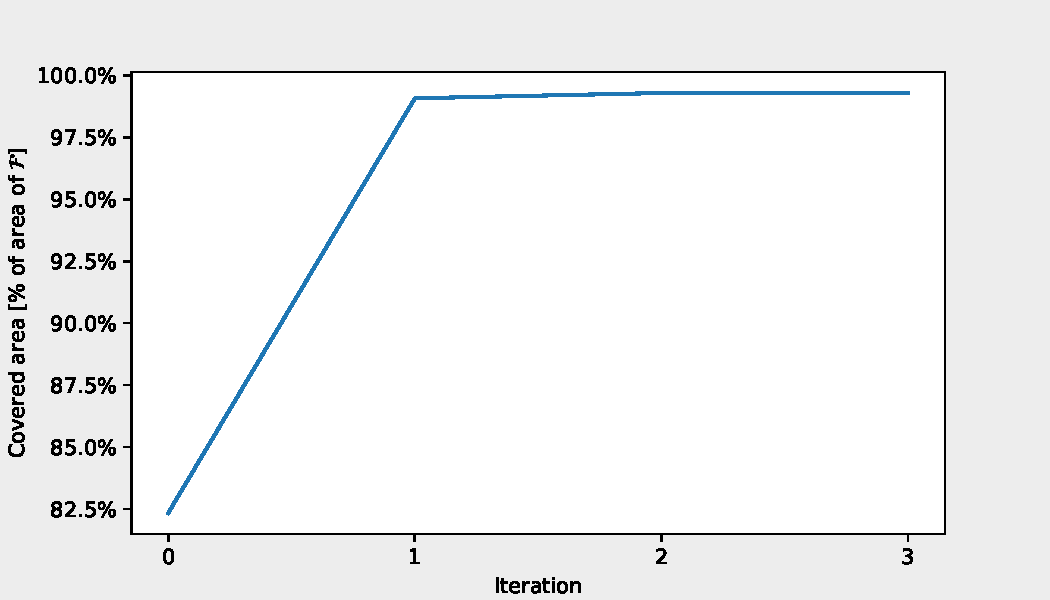
\includegraphics[width=\textwidth]{figs/tinyworld2_6_agnt_k_1_0_k_2_1_area_traj.pdf}
    \caption{Coverage evolution for 6 agents in the Tinyworld2 environment with $k_{1} = 0$ (no active dispersion).}
    \label{fig:6_agnt_tw2_k_1_0_a_traj}
  \end{subfigure}%
  ~ 
  \begin{subfigure}[t]{0.5\textwidth}
    \centering
    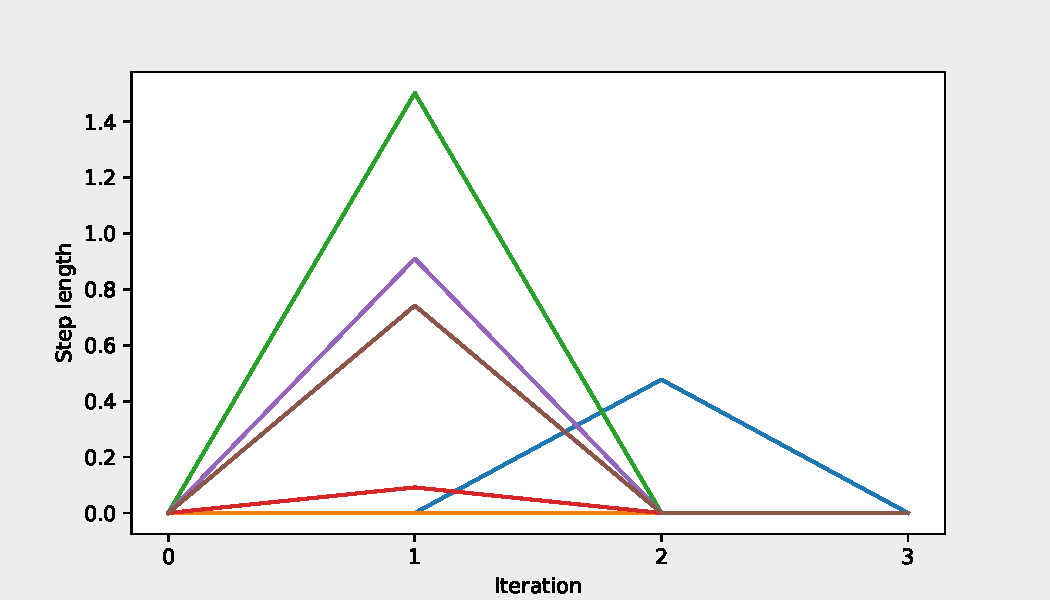
\includegraphics[width=\textwidth]{figs/tinyworld2_6_agnt_k_1_0_k_2_1_step_traj.pdf}
    \caption{Step length evolution for 6 agents in the Tinyworld2 environment with $k_{1} = 0$ (no active dispersion).}
    \label{fig:6_agnt_tw2_k_1_0_s_traj}
  \end{subfigure}
  \caption{Coverage percentage and step length evolution for 6 agents in the Tinyworld2 environment when active dispersion is not applied.}
  \label{fig:6_agnt_tw2_evolution}
\end{figure}

\begin{figure}[H]
  \centering
  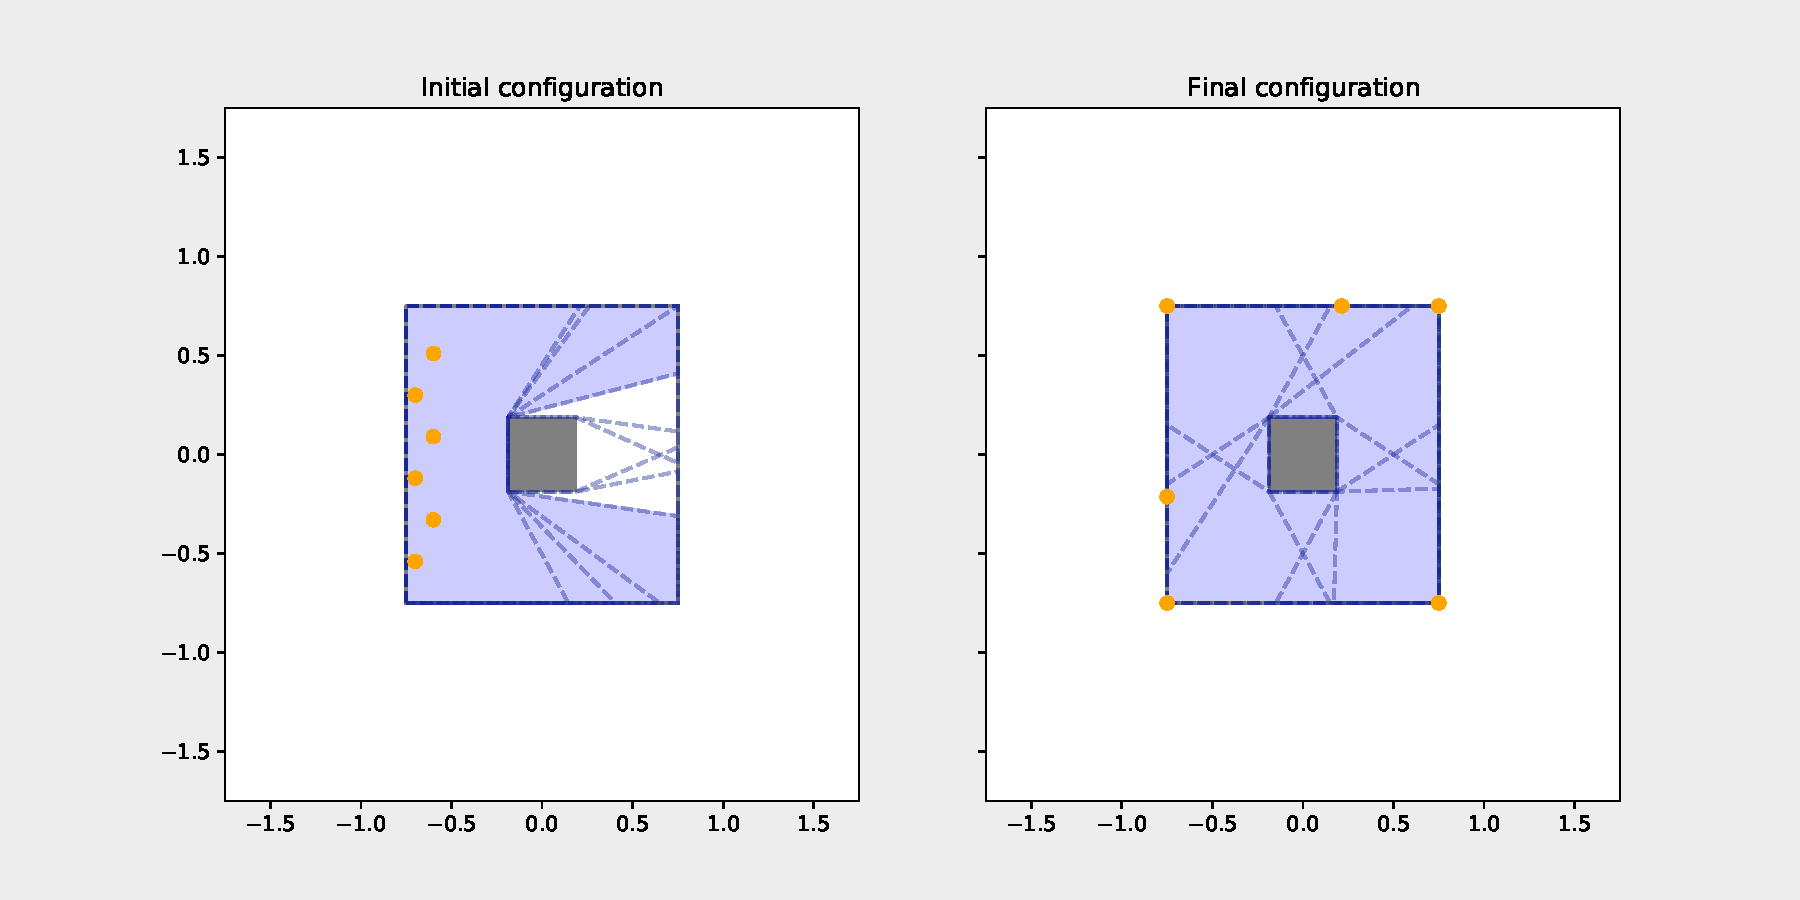
\includegraphics[width=\textwidth]{figs/tinyworld2_6_agnt_k_1_1_k_2_1_distr.pdf}
  \caption{Inital and final configuration of 6 agents in the Tinyworld2 environment with $k_{1} = k_{2} = 1$ (active dispersion).}
  \label{fig:6_agnt_tw2_k_1_1_k_2_1_distr}
\end{figure}
\begin{figure}[H]
  \centering
  \begin{subfigure}[t]{0.5\textwidth}
    \centering
    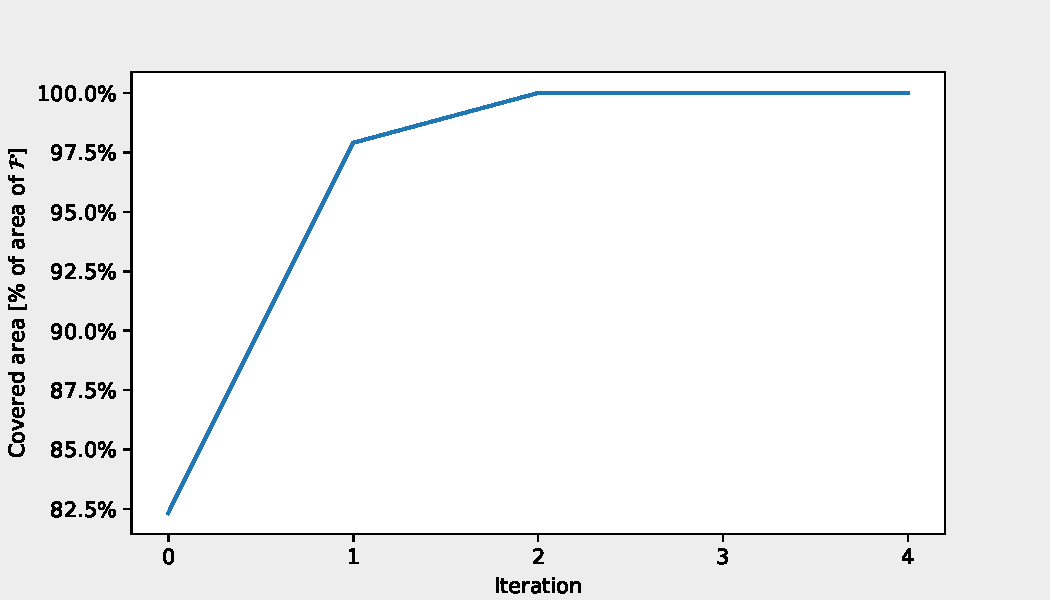
\includegraphics[width=\textwidth]{figs/tinyworld2_6_agnt_k_1_1_k_2_1_area_traj.pdf}
    \caption{Coverage evolution for 6 agents in the Tinyworld2 environment with $k_{1} = k_{1} = 1$ (active dispersion).}
    \label{fig:6_agnt_tw2_k_1_1_a_traj}
  \end{subfigure}%
  ~ 
  \begin{subfigure}[t]{0.5\textwidth}
    \centering
    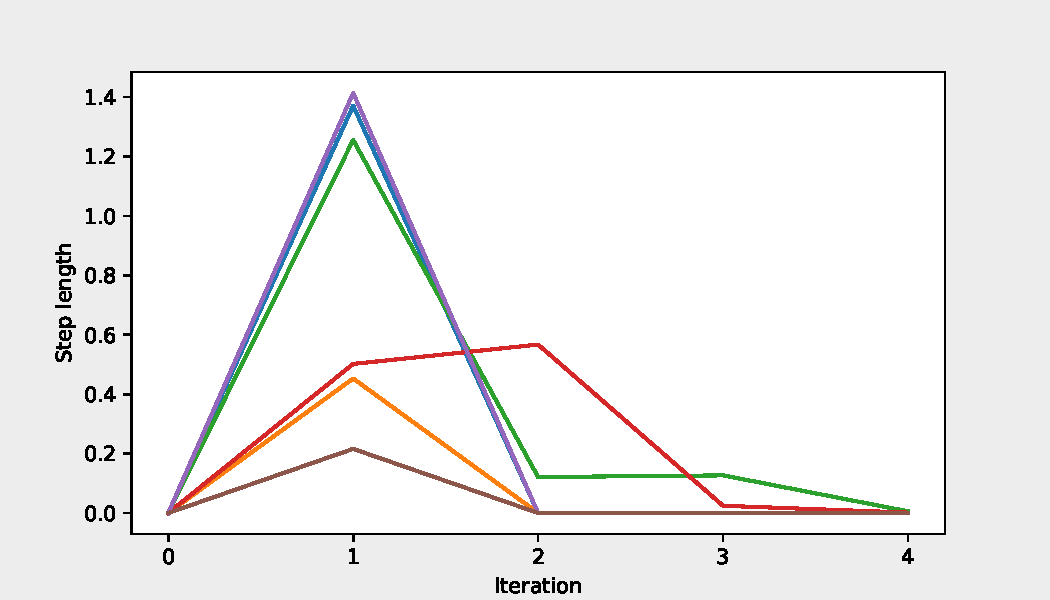
\includegraphics[width=\textwidth]{figs/tinyworld2_6_agnt_k_1_1_k_2_1_step_traj.pdf}
    \caption{Step length evolution for 6 agents in the Tinyworld2 environment with $k_{1} = k_{2} = 1$ (active dispersion).}
    \label{fig:6_agnt_tw2_k_1_1_s_traj}
  \end{subfigure}
  \caption{Coverage percentage and step length evolution for 6 agents in the Tinyworld2 environment when active dispersion is applied.}
  \label{fig:6_agnt_tw2_evolution_active}
\end{figure}
